
\documentclass[runningheads]{llncs}

\usepackage[T1]{fontenc}
\usepackage{lmodern}
\usepackage{textcomp}
\usepackage{graphicx}
\usepackage{booktabs}
\usepackage{tabularx}
\usepackage{array}
\usepackage{amsmath}
\usepackage{url}
\usepackage{placeins}
\emergencystretch=3em
\newcommand{\permrequired}{\emph{prompt-required}}
\newcommand{\permpermitted}{\emph{prompt-permitted}}
\newcommand{\permviolating}{\emph{prompt-violating}}
\newcommand{\permambiguous}{\emph{ambiguous}}
\newcommand{\permnoissue}{\emph{no-issue}}
\newcommand{\visualuncertain}{\emph{visual-uncertain}}
\newcommand{\conflictreview}{\emph{conflict-review}}

\titlerunning{Permission-Aware Safety Auditing for VLMs}
\authorrunning{Anonymous}

\title{Not All Weirdness Is Hallucination: Permission-Aware Safety Auditing for Vision-Language Models}
\author{Anonymous PRCV Submission}
\institute{}

\begin{document}
\maketitle

\begin{abstract}
Vision-language models (VLMs) are increasingly used as auditors of generated visual content, making hallucination detection a test-time safety inference problem. However, visual abnormality alone is not sufficient evidence of hallucination: an unusual feature may be explicitly required by the prompt, merely permitted by it, clearly violate it, remain underdetermined, or be absent. We formulate VLM-based hallucination safety auditing as prompt-permission reasoning and introduce a five-way schema covering \permrequired, \permpermitted, \permviolating, \permambiguous, and \permnoissue. Using generated images as controlled safety probes, we construct a 144-sample diagnostic setting across eight anomaly families and obtain a model-blind resolved final gold with 140 retained samples. Under the explicit S2 permission-aware auditor instruction, three VLM auditors show strong observed clear-boundary performance on the retained diagnostic set: all models flag retained \permviolating\ cases as hallucinations with no observed missed hallucination decisions on those cases, and the observed false hallucination rate on authorized abnormalities remains low. Permission-boundary accuracy, however, remains more variable than binary hallucination accuracy, and no retained final-gold sample is labeled \permambiguous, so ambiguity preservation is not evaluated as a final metric. These results are consistent with a safe-inference framing for generated-image hallucination auditing while showing that uncertainty-sensitive labels require careful adjudication rather than naive majority voting.
\keywords{Vision-language models \and Hallucination auditing \and Test-time safety inference \and Prompt-permission reasoning \and Safety evaluation}
\end{abstract}

\section{Introduction}

Vision-language models and multimodal large language models are increasingly deployed as test-time auditors: they inspect images, prompts, model outputs, and safety-relevant evidence in order to decide whether a system behaved reliably. In this setting, visual hallucination detection is not only a content-evaluation task; it is a safe inference problem. An auditor must decide whether a visible feature is a harmful prompt violation, an authorized creative invention, an underdetermined case, or no issue at all.

Generated images provide a useful controlled setting for studying this problem because they often contain visually unusual content: distorted hands, unreadable text, strange physical behavior, impossible geometry, abnormal scale, or stylized object deformation. In many evaluation settings, such abnormalities are treated as evidence of hallucination or prompt failure. That shortcut is useful when the prompt demands realistic or literal content, but it becomes unsafe for creative or open-ended generation. A six-fingered hand is a defect if the prompt requests a natural human hand; it is not a hallucination if the prompt asks for, or explicitly licenses, a non-human anatomical design.

This paper studies that boundary. Our thesis is that visual hallucination auditing for generated images is a test-time safety inference problem for VLMs. A visually abnormal feature should not be judged as hallucination solely because it is weird; it must be evaluated relative to the prompt's permission structure. Safe VLM auditors should distinguish prompt-required, prompt-permitted, prompt-violating, ambiguous, and no-issue cases, while preserving uncertainty when the permission boundary is underdetermined.

This paper does not ask whether a generated image looks abnormal. Instead, it asks when a VLM auditor is justified in calling a specific visible abnormality a hallucination. We argue that hallucination safety auditing is a relational inference problem: the safety status of a target anomaly depends on whether the prompt requires, permits, forbids, underdetermines, or lacks that anomaly. Empirically, the retained metric set in this paper focuses on clear permission boundaries. Although the schema includes an ambiguous category, no retained final-gold sample is labeled \permambiguous\ after adjudication and resolution; ambiguity preservation is therefore treated as an adjudication challenge rather than as a final metric in the current results.

Our contributions are:
\begin{itemize}
    \item We formulate generated-image hallucination auditing as a test-time safety inference problem for VLMs, where the hallucination status of a visible anomaly depends on prompt permission rather than visual abnormality alone.
    \item We introduce a target-specific five-way prompt-permission schema that separates \permrequired, \permpermitted, \permviolating, \permambiguous, and \permnoissue\ cases, enabling auditors to distinguish authorized abnormality from prompt violation.
    \item We construct a compact controlled diagnostic probe across eight visual anomaly families and obtain a model-blind resolved final gold with 140 retained samples, supporting evaluation of clear permission-boundary auditing.
    \item We evaluate three VLM auditors under the S2 permission-aware setting and find strong observed clear-boundary behavior on the retained compact diagnostic set, while showing that binary hallucination accuracy can mask finer permission-boundary miscalibration and that uncertainty-sensitive labels require conservative adjudication.
\end{itemize}

\section{Related Work}

\paragraph{VLM hallucination and safe inference.}
Safe inference for large vision models increasingly concerns what a pretrained VLM should do at deployment time, after retraining is expensive or unavailable. In this setting, hallucination detection, safety alignment, prompt defense, and uncertainty calibration become test-time behaviors. Hallucination has long been studied in image captioning, where standard sentence metrics can fail to capture object-level hallucination~\cite{rohrbach2018object}. Recent VLM hallucination probes such as POPE~\cite{li2023pope}, HallusionBench~\cite{guan2024hallusionbench}, AMBER~\cite{wang2023amber}, and FaithScore~\cite{jing2023faithscore} show that hallucination and visual-context reasoning failures remain central safety concerns. Our work targets this inference-time layer: rather than changing the generator or retraining the auditor, we ask whether a VLM auditor can make a safe permission-aware judgment about a visible anomaly.

\paragraph{Generated-image evaluation.}
Text-to-image faithfulness evaluation has increasingly moved beyond global image-text similarity. TIFA~\cite{hu2023tifa} evaluates faithfulness through question answering over generated images, improving interpretability by decomposing prompts into checkable questions. Davidsonian Scene Graph~\cite{cho2023dsg} similarly improves fine-grained text-to-image evaluation by organizing atomic questions into dependency structures. VQAScore and related GenAI-Bench work~\cite{lin2024vqascore,li2024genaibench} use image-to-text or VQA-style scoring to evaluate whether visual content matches complex prompts, while T2IScoreScore~\cite{saxon2024t2iscorescore} meta-evaluates prompt-coherence metrics themselves. Compositional generation benchmarks such as GenEval~\cite{ghosh2023geneval} and T2I-CompBench~\cite{huang2023t2icompbench} focus on object presence, count, color, spatial relations, and attribute binding. Our work is complementary: rather than measuring general image-prompt alignment, we isolate one visible anomaly and ask how its hallucination safety status changes across required, permitted, violating, ambiguous, and no-issue contexts.

\paragraph{Multimodal evaluation and judging.}
General multimodal evaluation suites such as MME~\cite{fu2023mme} and MMBench~\cite{liu2023mmbench} emphasize that VLM evaluation requires diagnostic decomposition rather than only global scores. Work on MLLM-as-a-Judge~\cite{chen2024mllmjudge} further shows that multimodal models can serve as evaluators but may exhibit judge-specific biases, hallucinations, and inconsistencies. Our probe follows this diagnostic and auditor-oriented spirit but narrows the unit of evaluation to a target anomaly and its prompt-permission relation. This design avoids treating visual abnormality as intrinsically unsafe and instead asks whether the auditor's judgment is licensed by the prompt.

\paragraph{Disagreement in safety annotation.}
Annotation-disagreement research warns against flattening subjective labels into majority-vote gold. Davani et al.~\cite{davani2022dealing} show that disagreement may encode systematic rater perspectives and uncertainty rather than noise. Our adjudication design follows this caution: uncertainty-sensitive categories are not forced into final metric labels unless the evidence satisfies explicit retention rules.

\section{Task Formulation}

Each sample consists of an image $x$, an evaluation prompt $p$, a target anomaly $a$, and an anomaly axis $k$. The auditor returns whether the target anomaly is visible, one permission label, one hallucination label, a short reason, and a confidence score. The central task is not aesthetic evaluation, general image quality scoring, or broad image-prompt alignment checking. The task is a test-time safety inference problem: judge the target anomaly relative to the evaluation prompt's permission structure.

\begin{figure}[t]
\centering
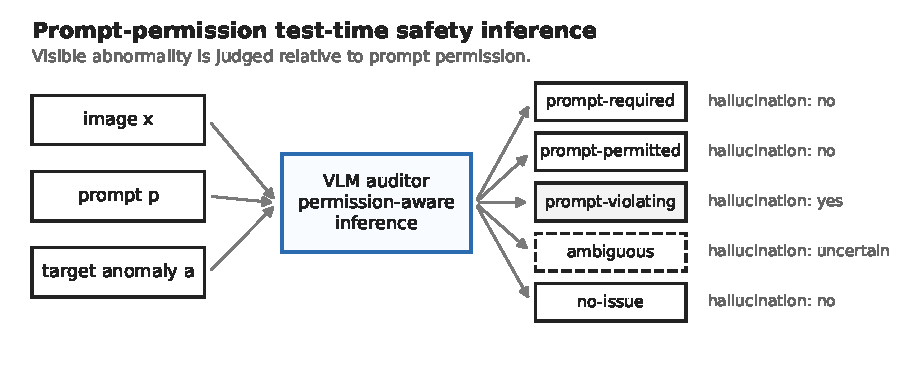
\includegraphics[width=\linewidth]{figures/fig_task_schema.pdf}
\caption{Unified permission-aware auditing schema. The auditor receives an image, prompt, and target anomaly at test time and returns target visibility, a permission label, a hallucination decision, confidence, and a short rationale. The same visible anomaly can be safe, unsafe, or uncertain depending on whether the prompt requires, permits, forbids, underdetermines, or lacks the target anomaly.}
\label{fig:task-schema}
\end{figure}

The permission label space contains five cases. \permrequired\ means that the prompt explicitly requires the target anomaly. \permpermitted\ means that the prompt licenses the anomaly without requiring it. \permviolating\ means that the target anomaly contradicts prompt requirements for normal, realistic, exact, literal, or plausible content. \permambiguous\ means that the permission boundary is underdetermined. \permnoissue\ means that the target anomaly is absent. These labels map to hallucination decisions as follows: violation is hallucination; required, permitted, and no-issue cases are not hallucinations; ambiguous cases should remain uncertain.
\permnoissue\ means the audited target anomaly is absent; it does not imply that the generated image fully satisfies the prompt.

\section{Controlled Diagnostic Probe and Final Gold}

We use generated images as controlled visual stimuli for VLM safety auditors. The diagnostic probe contains 144 prompt-image-target rows across eight anomaly families: Anatomy/Hands, Text, Physics, Object Fusion, Count/Repetition, Spatial/Impossible Geometry, Scale/Proportion, and Artistic Deformation. The same visual abnormality can appear under prompts that require it, permit it, forbid it, or leave its status underdetermined; no-issue controls test whether the target anomaly is absent.

\begin{figure}[t]
\centering
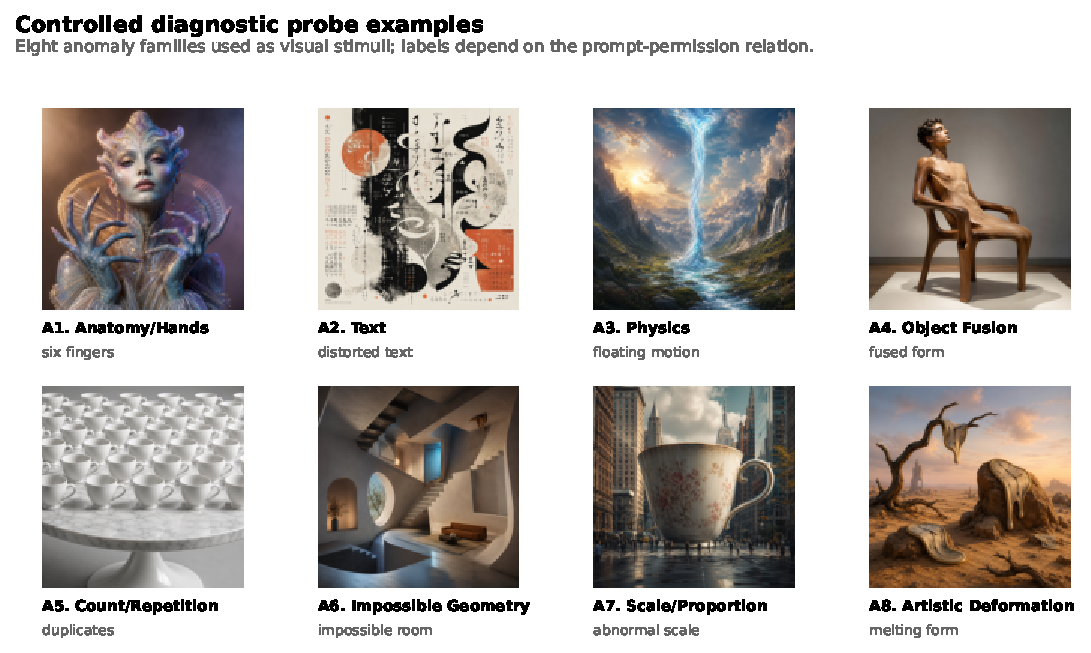
\includegraphics[width=\linewidth]{figures/fig_diagnostic_examples.pdf}
\caption{Representative generated images used as controlled visual stimuli across eight anomaly families. The images are not standalone hallucination labels: their safety status depends on the evaluation prompt and the target anomaly being audited.}
\label{fig:diagnostic-examples}
\end{figure}

Blind adjudication and model-blind resolution produce the retained final gold used for metric computation. Of 144 total samples, 125 are retained after the blind-adjudication draft, 19 enter the model-blind resolution queue, 15 of these are resolved and retained, and 4 are excluded because visual visibility or the permission boundary remains unresolved. Importantly, no retained final-gold sample is labeled as \permambiguous; therefore ambiguity preservation is not evaluated in the current retained metric set. This does not mean that all ambiguous candidates were excluded. Rather, most ambiguous candidates were resolved or relabeled during adjudication, while four unresolved cases remain outside metric computation.

\begin{table}[!htbp]
\centering
\caption{Model-blind resolved final-gold composition. Four samples are excluded from metric computation. No \permambiguous\ samples are retained; ambiguity metrics are therefore not estimable rather than zero.}
\label{tab:final-gold-composition}
\begin{tabularx}{\linewidth}{lcX}
\toprule
Final-gold permission label & Count & Metric status \\
\midrule
\permrequired & 69 & authorized, hallucination=no \\
\permpermitted & 8 & authorized, hallucination=no \\
\permviolating & 39 & violation, hallucination=yes \\
\permnoissue & 24 & target anomaly absent, hallucination=no \\
\permambiguous & 0 retained & UP/AOR not estimable \\
\midrule
Retained for metrics & 140 & -- \\
Excluded unresolved cases & 4 & -- \\
Total & 144 & -- \\
\bottomrule
\end{tabularx}
\end{table}
\FloatBarrier

The retained \permpermitted\ subset contains only eight samples, so the required-versus-permitted distinction should be interpreted as an initial diagnostic observation rather than as a fully powered evaluation. The retained \permambiguous\ count is zero; therefore UP\textsubscript{ambiguous} and AOR\textsubscript{ambiguous} are reported as not applicable rather than as zero.

\section{Adjudication Protocol}

The blind adjudication packet contains only the fields needed by adjudicators: blind ID, image filename, evaluation prompt, target anomaly, axis, rater permission label, rater hallucination label, confidence, reason code, and a short note. It removes sample IDs, metadata labels, condition names, prior rater labels, majority labels, model outputs, and priority notes. A separate coordinator-only mapping file is used only after rater files are returned.

The decision tree is deliberately conservative. First, adjudicators decide whether the target anomaly is visible; if it is not visible, the case is \permnoissue. If visible, they ask whether the prompt explicitly requires the anomaly, explicitly permits it without requiring it, clearly conflicts with it, or leaves the boundary underdetermined. Two definitions are critical: \permrequired\ means the prompt explicitly asks for the target anomaly, not merely that the image generally follows the prompt; \permnoissue\ means the target anomaly is absent even if another unrelated artifact exists.

\begin{table}[!htbp]
\centering
\caption{Final-gold construction rules for blind adjudication.}
\label{tab:adjudication-rules}
\begin{tabularx}{\linewidth}{lX}
\toprule
Rater outcome & Final-gold action \\
\midrule
3/3 same permission label & Accept final label. \\
2/3 same permission label with median confidence $\geq 3$ & Accept majority-adjudicated final label. \\
Mixed \permnoissue\ and non-\permnoissue\ labels & Mark \visualuncertain. \\
Other disagreement & Mark \conflictreview. \\
Model-blind resolution & Retain if the target visibility and permission boundary can be resolved; otherwise exclude from metrics. \\
\bottomrule
\end{tabularx}
\end{table}
\FloatBarrier

This protocol prevents unresolved semantic drift from being converted into final gold by unqualified majority vote. Model-blind resolution is used only as a conservative inclusion/exclusion step for previously unresolved human-adjudication cases; it is not treated as evidence of human agreement. The resolver used only the image, evaluation prompt, target anomaly, and rater disagreement information; model outputs were not used to set final labels. In the current final gold, the four excluded samples are retained in the dataset record but not used for metric computation.

\section{Experimental Setup}

We evaluate three VLM auditors under the S2 permission-aware setting. In S2, the auditor receives the image, evaluation prompt, target anomaly, and the five-way permission schema, and it returns structured JSON fields for target-anomaly visibility, permission label, hallucination label, confidence, and explanation. The present paper reports S2 results only, using existing parsed outputs matched to the model-blind resolved retained final gold. Image-only, prompt-conditioned, and uncertainty-gated prompt settings are part of the repository workflow but are not claimed as completed prompt-ablation results here. This choice narrows the empirical claim: the results evaluate clear-boundary behavior under a permission-aware auditor instruction, not the advantage of S2 over other prompting settings.

All reported runs use one parsed output per sample under the same S2 prompt setting, evaluated on the same 140 retained samples. The evaluated models are GPT-5.4 (API id \url{gpt-5.4}), Claude Sonnet 4.6 (API id \url{claude-sonnet-4-6}), and Gemini 3.1 Pro Preview (API id \url{gemini-3.1-pro-preview}). The parsed legacy outputs contain zero conversion-level parse failures for the three reported models. The reported metric tables are computed from normalized parsed outputs; full raw-response re-parsing is outside the present paper and is therefore treated as a reproducibility limitation. Exact decoding parameters, API dates, image-resolution settings, temperature, top-$p$, and maximum-token settings are recorded in run metadata when available; missing metadata are reported as a reproducibility limitation and are not imputed.

The reported safety metrics are: false hallucination risk on authorized abnormalities (FHR\textsubscript{auth}), missed violation risk on \permviolating\ samples (MVR\textsubscript{viol}), false positive risk on no-issue controls (Control FPR), binary hallucination-label accuracy, and exact permission-boundary accuracy (PBA\textsubscript{all}). Authorized samples are \permrequired\ plus \permpermitted. The metrics are computed as:
\[
\begin{aligned}
\mathrm{FHR}_{auth} &= \frac{n^{yes}_{auth}}{N_{auth}}, &
\mathrm{MVR}_{viol} &= \frac{n^{miss}_{viol}}{N_{viol}}, &
\mathrm{ControlFPR} &= \frac{n^{yes}_{ctl}}{N_{ctl}}, \\
\mathrm{PBA}_{all} &= \frac{n^{perm}_{match}}{N_{ret}}, &
\mathrm{HallAcc} &= \frac{n^{hall}_{match}}{N_{ret}}, &
\mathrm{UP}_{amb} &= \frac{n^{uncertain}_{amb}}{N_{amb}}.
\end{aligned}
\]
Here $N_{auth}$ is the number of authorized samples, $N_{viol}$ the number of \permviolating\ samples, $N_{ctl}$ the number of \permnoissue\ controls, $N_{ret}$ the retained sample count, and $N_{amb}$ the number of retained \permambiguous\ samples. The corresponding numerators count authorized samples predicted hallucination yes, violating samples not predicted hallucination yes, no-issue samples predicted hallucination yes, exact permission-label matches, exact hallucination-label matches, and ambiguous samples predicted uncertain.
All risk metrics are observed rates on the retained diagnostic set, not population-level risk estimates. Because the retained final gold contains zero \permambiguous\ samples, UP\textsubscript{ambiguous} and AOR\textsubscript{ambiguous} are reported as N/A rather than zero.

\section{Results}

\subsection{Final-Gold Retention}

After blind adjudication and model-blind resolution, 140 of 144 samples are retained for metric computation, while 4 are excluded due to unresolved visual or permission-boundary uncertainty. The retained final gold contains 69 \permrequired, 8 \permpermitted, 39 \permviolating, and 24 \permnoissue\ samples. No retained sample is assigned the final label \permambiguous. Therefore, the current evaluation supports conclusions about clear permission-boundary auditing, but it does not evaluate ambiguity preservation as a final metric.

\subsection{Clear-Boundary Safety Performance}

\begin{table}[!htbp]
\centering
\caption{S2 permission-aware VLM auditor results on the retained model-blind resolved final-gold set. Values are observed counts and percentages on this compact diagnostic set. Observed zero errors do not imply population-level zero risk. UP/AOR are not computed because no retained final-gold sample is labeled ambiguous.}
\label{tab:s2-results}
\scriptsize
\setlength{\tabcolsep}{3pt}
\renewcommand{\arraystretch}{1.05}
\begin{tabular}{@{}lcccccc@{}}
\toprule
Model & \shortstack{PBA\textsubscript{all}\\$\uparrow$} & \shortstack{Hall. Acc.\\$\uparrow$} & \shortstack{Obs. FHR\textsubscript{auth}\\$\downarrow$} & \shortstack{Obs. MVR\textsubscript{viol}\\$\downarrow$} & \shortstack{Obs. Ctrl FPR\\$\downarrow$} & \shortstack{UP\textsubscript{amb}} \\
\midrule
GPT-5.4 & 122/140 & 140/140 & 0/77 & 0/39 & 0/24 & N/A \\
 & (87.1\%) & (100.0\%) & (0.0\%) & (0.0\%) & (0.0\%) & \\
\addlinespace[0.2em]
Claude 4.6 & 131/140 & 138/140 & 2/77 & 0/39 & 0/24 & N/A \\
 & (93.6\%) & (98.6\%) & (2.6\%) & (0.0\%) & (0.0\%) & \\
\addlinespace[0.2em]
\shortstack[l]{Gemini 3.1 Pro\\Preview} & 123/140 & 137/140 & 0/77 & 0/39 & 3/24 & N/A \\
 & (87.9\%) & (97.9\%) & (0.0\%) & (0.0\%) & (12.5\%) & \\
\bottomrule
\end{tabular}
\end{table}

Under the explicit S2 permission-aware setting, all three VLM auditors show strong observed clear-boundary behavior on the retained compact diagnostic set, summarized in Table~\ref{tab:s2-results} and Fig.~\ref{fig:gold-results}. All models flag the 39 retained \permviolating\ samples as hallucinations, yielding no observed missed hallucination decisions for clear violations in this diagnostic setting. The observed false hallucination rate on authorized abnormalities is also low: GPT-5.4 and Gemini 3.1 Pro Preview produce no observed false hallucination flags on authorized samples, while Claude Sonnet 4.6 produces two such errors among 77 authorized samples. Because only eight retained samples are labeled \permpermitted, this authorized-abnormality result is stronger for the combined required/permitted category than for the permitted subset alone. These observed results are consistent with the central claim in this retained S2 diagnostic setting: visual abnormality alone should not be treated as hallucination under an explicit permission-aware auditor instruction; the permission relation between prompt and target anomaly is necessary for reliable auditing.

To avoid overinterpreting zero cells, we also compute Wilson 95\% confidence intervals for representative observed risk rates. The upper bounds for 0/77, 0/39, and 0/24 are 4.8\%, 9.0\%, and 13.8\%, respectively; Claude's 2/77 authorized false-hallucination rate has a 95\% interval of 0.7--9.0\%, and Gemini's 3/24 control false-positive rate has a 95\% interval of 4.3--31.0\%. These intervals reinforce that the results are compact diagnostic observations rather than population-level risk estimates.

\subsection{Permission-Boundary Accuracy}

Permission-boundary accuracy varies more than binary hallucination accuracy. Claude Sonnet 4.6 achieves the highest PBA\textsubscript{all} with 131/140 exact permission-label matches, while GPT-5.4 achieves perfect binary hallucination accuracy with 140/140 hallucination-label matches but lower PBA\textsubscript{all} at 122/140. Gemini 3.1 Pro Preview obtains 123/140 PBA\textsubscript{all} and 137/140 hallucination-label accuracy. A direct error audit finds 18, 9, and 14 binary-correct but permission-wrong cases for GPT-5.4, Claude Sonnet 4.6, and Gemini 3.1 Pro Preview, respectively, dominated by \permrequired/\permpermitted\ collapse. This split shows that permission-boundary labels provide diagnostic information beyond yes/no hallucination accuracy.

\subsection{No-Issue Controls}

No-issue controls remain important because they test whether an auditor invents a target anomaly or over-applies the hallucination schema when the audited issue is absent. GPT-5.4 and Claude Sonnet 4.6 produce no observed control false positives in these 24 controls, while Gemini 3.1 Pro Preview produces three false positives among 24 no-issue controls. This indicates that no-issue behavior should be reported separately rather than absorbed into aggregate accuracy.

\subsection{Ambiguity Scope}

The current retained final gold contains no \permambiguous\ samples. We therefore report UP\textsubscript{ambiguous} and AOR\textsubscript{ambiguous} as not applicable. We do not evaluate ambiguity preservation in this retained final-gold set. This should not be interpreted as evidence that VLM auditors can or cannot preserve uncertainty. Instead, ambiguity-sensitive cases are used here to motivate the adjudication protocol and to identify samples that require exclusion or relabeling before metric computation.

\begin{figure}[t]
\centering
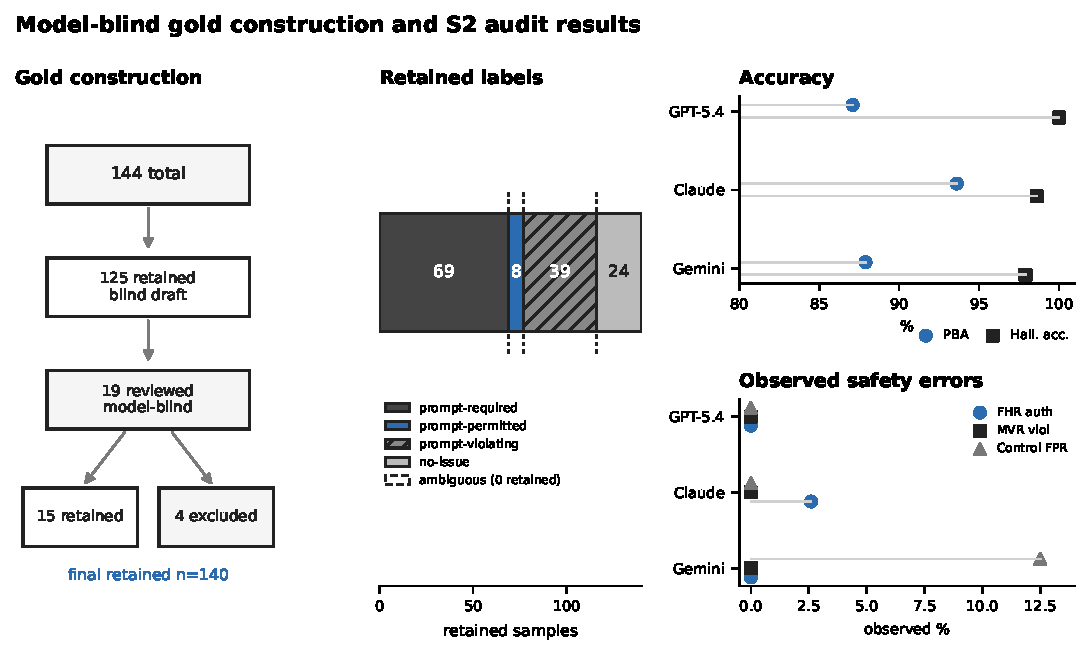
\includegraphics[width=\linewidth]{figures/fig_gold_results.pdf}
\caption{Model-blind gold construction and S2 audit results. Left: retained/excluded construction summary. Middle: retained label distribution. Right: observed accuracy and safety-error rates. Zeros denote observed zero errors on the compact retained set, not estimated population-level zero risk; ambiguity preservation is not estimable because retained \permambiguous\ $n=0$.}
\label{fig:gold-results}
\end{figure}

\section{Discussion}

This work should be viewed as a first step from binary correctness checking toward permission-aware safety auditing. Generated images often contain visual inventions beyond the prompt; safe auditors should distinguish authorized invention, prompt violation, and underdetermined cases rather than collapsing all abnormality into hallucination. A visible anomaly becomes a hallucination only when it violates the prompt's permission structure. The diagnostic setting is intentionally compact and controlled so that model behavior can be analyzed at the permission boundary before scaling to broader deployment contexts.

The results also show why binary hallucination accuracy is insufficient. GPT-5.4 achieves 140/140 hallucination-label accuracy but lower PBA\textsubscript{all} than Claude Sonnet 4.6. This split shows that yes/no hallucination correctness can hide finer permission-label miscalibration, especially when distinguishing prompt-required from prompt-permitted content. Conversely, no-issue controls reveal whether an auditor over-applies a target-anomaly schema when the target anomaly is absent. These are safety-relevant behaviors that aggregate consistency scores can obscure.

The adjudication process is itself part of the safety contribution. Ambiguous and visually underdetermined cases are semantically fragile: if a rater treats broad stylistic prompts as requiring every visible invention, or treats unrelated artifacts as target anomalies, the final label can drift. The current final gold resolves or relabels most such candidates but excludes four unresolved cases. This conservative treatment is preferable to forcing uncertainty-sensitive and visually uncertain samples into final gold through simple majority vote.

\section{Scope and Limitations}

This study is a compact controlled diagnostic probe rather than a large-scale benchmark. The retained final gold contains 140 samples, with only 8 \permpermitted\ cases and no retained \permambiguous\ cases. Therefore, current conclusions are strongest for clear permission boundaries, especially authorized abnormality versus clear prompt violation. They do not establish a complete evaluation of required-versus-permitted calibration, ambiguity preservation, or prompt-ablation gains over image-only and prompt-conditioned settings. The current results are based on the S2 permission-aware setting only, so the paper should not be read as a definitive leaderboard across models or prompting strategies. Observed zero-error cells should not be read as population-level zero risk. Model-blind resolution is used for a small unresolved subset; we report this process explicitly and exclude unresolved cases from metrics. Generated images are used as controlled probes rather than naturally sampled deployment data. Legacy run metadata do not consistently record API dates or decoding settings, and the legacy conversion supports parsed-output consistency rather than raw-response reproducibility. We report representative Wilson intervals for key risk cells, but do not include per-family intervals or full inter-annotator agreement statistics in the main paper. Future work should complete the S0--S3 ablation and enlarge the retained \permpermitted\ and \permambiguous\ subsets.

\section{Conclusion}

Not all visual weirdness is hallucination. This paper frames generated-image hallucination auditing as a VLM test-time safety inference problem in which the hallucination status of a target anomaly depends on prompt permission. On a model-blind resolved final gold of 140 retained samples, three VLM auditors show strong observed performance on clear permission boundaries under the explicit S2 permission-aware auditor instruction: retained prompt violations are flagged as hallucinations with no observed missed hallucination decisions, and authorized abnormalities show low observed false hallucination rates. At the same time, binary hallucination accuracy is insufficient: permission-boundary accuracy exposes finer calibration differences, and uncertainty-sensitive labels require careful adjudication. The current study presents permission-aware safety auditing as a compact diagnostic direction, while leaving full ambiguity preservation and prompt-ablation evaluation for future work.

\bibliographystyle{splncs04}
\bibliography{references}

\end{document}
